\section{Les fragments}
Permet d'afficher plusieurs vues sur un écran. Ces fragments permettent une modularité, et donc, une réutilisabilité. On peut donc éviter de créer une activité par vue, l'utilisateur peut mieux naviguer ainsi.

Seul problème, ce n'est supporté qu'à partie de Honeycomp (Android 3.0, API 11). Il faut donc utiliser la librairie \code{android.support.v4.app.FragmentActivity}, pour être compatible avec les versions antérieures.

\subsection{Les différents types de fragments}
Il est possible d'utiliser les sous-classes suivantes de \code{Fragment} :
\begin{itemize}
    \item \code{DialogFragment}, une fenêtre de dialogue flottante ;
    \item \code{ListFragment}, une liste d’éléments ;
    \item \code{PreferenceFragment}, une liste de préférences.
\end{itemize}

\subsection{Implantation}
\begin{figure}[H]
    \centering
    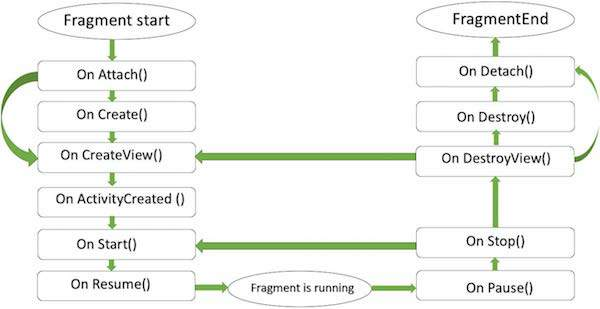
\includegraphics[width=.75\textwidth]{assets/fragment.jpg}
    \caption{Le cycle de vie de la classe \code{Fragment}.}
\end{figure}

\subsection{Exemple}
\begin{lstlisting}[language=java]
class TestFragment extends Fragment {
    @Override
    public void onCreate(Bundle savedInstanceState) {
        // TODO Auto-generated method stub
        super.onCreate(savedInstanceState);
    }
    
    @Override
    public View onCreateView(LayoutInflater inflater, ViewGroup container, Bundle savedInstanceState) {
        // TODO Auto-generated method stub
        return super.onCreateView(inflater, container, savedInstanceState);
    }
    
    @Override
    public void onPause() {
        // TODO Auto-generated method stub
        super.onPause();
    }
}
\end{lstlisting}

\subsection{Insertion d'un fragment dans un layout}
\subsubsection{De manière statique}
\begin{lstlisting}[language=xml]
<LinearLayout
    android:id="@+id/linearLayout1"
    android:layout_width="match_parent"
    android:layout_height="match_parent"
    android:layout_alignLeft="@+id/button2"
    android:layout_below="@+id/button2"
    android:layout_marginTop="54dp"
    android:orientation="vertical">
        <fragment android:id="@+id/fragment1"
            android:name="com.example.androidtp3.TestFragment"
            android:layout_width="wrap_content"
            android:layout_height="wrap_content"
            android:layout_centerHorizontal="true"
            android:layout_centerVertical="true" />
</LinearLayout>
\end{lstlisting}

\subsubsection{De manière dynamique}
\begin{lstlisting}[language=java]
FragmentManager manager = getSupportFragmentManager();
FragmentTransaction transaction = manager.beginTransaction();
TestFragment fragment = new TestFragment();

transaction.add(R.id.linearLayout1, fragment);
transaction.commit();
\end{lstlisting}

Dans le cas d'un fragment sans UI, on lui donnera manuellement un identifiant nous permettant de le récupérer plus tard.
\begin{lstlisting}[language=java]
TestFragment fragment = new TestFragment();

transaction.add(fragment, "fragmentId");
transaction.commit();
\end{lstlisting}

\subsection{La gestion de fragments}
On utilise la classe \code{FragmentManager} pour gérer les fragments d'une activité. Pour récupérer le gestionnaire, on fera :
\begin{lstlisting}
FragmentManager manager = getSupportFragmentManager()
\end{lstlisting}

On va ensuite pouvoir lister les fragments à l'aide des méthodes suivantes :
\begin{itemize}
    \item \code{manager.findFragmentById()}, récupère les fragments de l’activité qui ont une UI (l’ID donnée est l’identifiant du container dans lequel est attaché le fragment) ;
    \item \code{manager.findFragmentByTag()}, récupère les fragments de l’activité qui n’ont pas d’IU (recherche par chaîne de caractères).
\end{itemize}

\subsubsection{Transactions sur les fragments}
Grâce au gestionnaire \code{FragmentManager} on va pouvoir commencer des transactions sur les fragments à l'aide de \code{FragmentTransaction}. Pour cela, on fera :

\begin{lstlisting}[language=java]
FragmentTransaction transaction = manager.beginTransaction();
// add(), remove(), replace(), ...
transaction.commit();
\end{lstlisting}

\subsection{S'adapter à la taille et l'orientation de l'appareil}
\begin{itemize}
    \item \code{res/layout/main.xml} (défaut, recommandé pour les smartphones) ;
    \item \code{res/layout-normal/main.xml} ;
    \item \code{res/layout-large/main.xml} (tablettes) ;
    \item \code{res/layout-xlarge/main.xml}.
\end{itemize}
